\documentclass[compress,aspectratio=169]{beamer}
\usepackage[T1]{fontenc} % Codificación de salida (tipos con tilde) y silabación castellana
\usepackage[utf8]{inputenc} % Reconocer tildes
\usepackage[english, spanish, es-tabla]{babel} % Idiomas para silabación y castellano principal; "tabla" en lugar de "cuadro"
\usepackage{hyperref}
\usepackage{pgfpages}
\usepackage{enumitem} % Subapartados en itemize y enumerate
\usepackage{tikz}

\usetikzlibrary{mindmap}

%%%%%%%%%%%%% Itemize múltiple %%%%%%%%%%%%%%
\newlist{SubItemList}{itemize}{1}
\setlist[SubItemList]{label={$-$}}

\let\OldItem\item
\newcommand{\SubItemStart}[1]{%
	\let\item\SubItemEnd
	\begin{SubItemList}[resume]%
		\OldItem #1%
	}
	\newcommand{\SubItemMiddle}[1]{%
		\OldItem #1%
	}
	\newcommand{\SubItemEnd}[1]{%
	\end{SubItemList}%
	\let\item\OldItem
	\item #1%
}
\newcommand*{\SubItem}[1]{%
	\let\SubItem\SubItemMiddle%
	\SubItemStart{#1}%
}%
%%%%%%%%%%%%%%%%%%%%%%%%%%%%%%%%%%%%%%%%%%%%%

\mode<presentation>
{
	\usetheme{NYU}      % or try Darmstadt, Madrid, Warsaw, ...
	\usecolortheme{default} % or try albatross, beaver, crane, ...
	\usefonttheme{serif}  % or try serif, structurebold, ...
	\setbeamertemplate{navigation symbols}{}
	\setbeamertemplate{caption}[numbered]
	\setbeamertemplate{frametitle}[default][right]
	\setbeamertemplate{note page}[plain]
	\setbeameroption{show notes on second screen=right}
} 

\title[Baco]{Baco: \foreignlanguage{english}{\textit{streaming}} de vídeo y VoIP sobre TCP}
\subtitle{Trabajo de Fin de Ciclo}
\author{Carlos Clement Bellido}
\institute{IES Doctor Balmis, Alicante}
\date{\today}
\titlegraphic{\hfill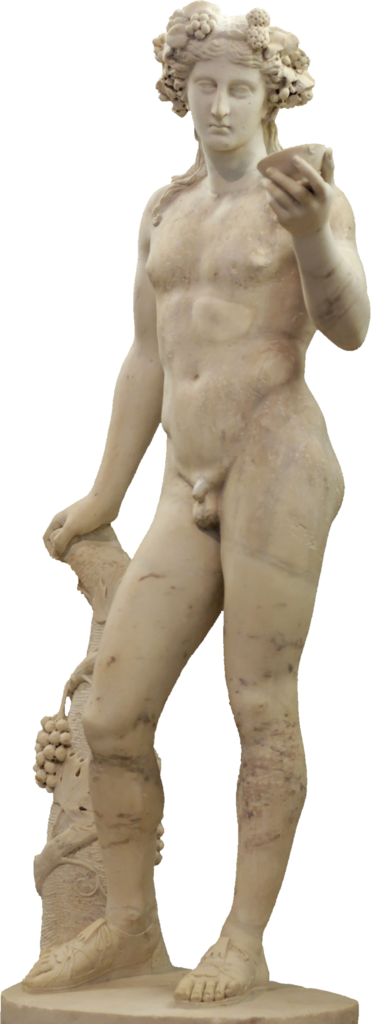
\includegraphics[height=1.5cm]{img/baco.png}}

\begin{document}
	
	
	\begin{frame} 
		
		\note{Hola, mi nombre es Carlos Clement Bellido y mi trabajo de fin de ciclo es una aplicación de \selectlanguage{english}\textit{streaming}\selectlanguage{spanish} de vídeo y transmisión de voz por protocolo de Internet sobre TCP.\\
			Al ser un programa que comunica usuarios por Internet se ha optado por un esquema de cliente -- servidor. El servidor posee un puerto conocido y es al que acceden todos los clientes.\\
			Vamos a ver en estas diapositivas cómo ocurren las comunicaciones entre el cliente, el servidor y la base de datos por Internet.} 
		
		\titlepage
	\end{frame}
	
	\begin{frame} 
		
		\note{A lo largo de esta exposición hablaremos de manera superficial de los siguientes apartados:
		\begin{enumerate}
			\item Baco -- Cliente: hablaremos de cómo se comporta la aplicación en el cliente
			\begin{itemize}
				\item Comunicación cliente -- servidor: su comunicación con el servidor
				\item Comunicación cliente -- base de datos: cómo accede al API REST (que veremos que no lo hace directamente)
			\end{itemize}
			\item BacoServer -- Servidor: en el servidor comentaremos cuál es su función
			\begin{itemize}
				\item Comunicación servidor -- cliente: cómo habla con el cliente y para qué
				\item Comunicación servidor -- base de datos: como se comunica con el API REST
			\end{itemize}
			\item API REST: veremos cómo maneja las peticiones y cómo modifica la base de datos
		\end{enumerate}}
		
		\tableofcontents
	\end{frame}

	\section{Baco -- Cliente}
	\begin{frame}{Baco -- Cliente}
		
		\note{Comenzaremos por la parte del cliente, el programa que se distribuirá. Tenemos dos pantallas únicamente, el lanzador y la ventana de la aplicación. En esta ventana transcurrirán todas las acciones y en la parte lateral izquierda podremos ir de pantalla en pantalla. Más adelante se hará una demostración gráfica de la aplicación.}
		
		\begin{columns}
			\column{0.5\textwidth}
			\begin{center}
				Lanzador de la aplicación
			\end{center}
			\begin{figure}
				\centering
				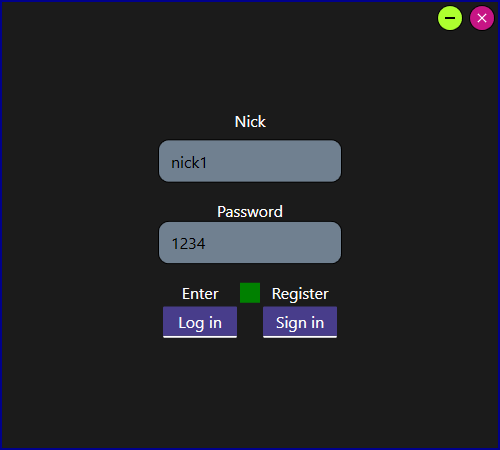
\includegraphics[width=0.5\textwidth,height=\textheight, keepaspectratio]{img/login.PNG}
			\end{figure}
			\begin{itemize}
				\item Registro
				\item Entrada con cuenta existente
			\end{itemize}
			\column{0.5\textwidth}
			\begin{columns}
				\column{0.5\textwidth}
				\begin{itemize}
					\item Llamadas
					\item Modificación del perfil
					\item Visor RSS
				\end{itemize}
				\column{0.5\textwidth}
				\begin{itemize}
					\item Mensajería
					\item Configuración
					\item Ver/hacer amigos
				\end{itemize}
			\end{columns}
			\begin{center}
				Pantalla principal de Baco
			\end{center}
			\begin{figure}
				\centering
				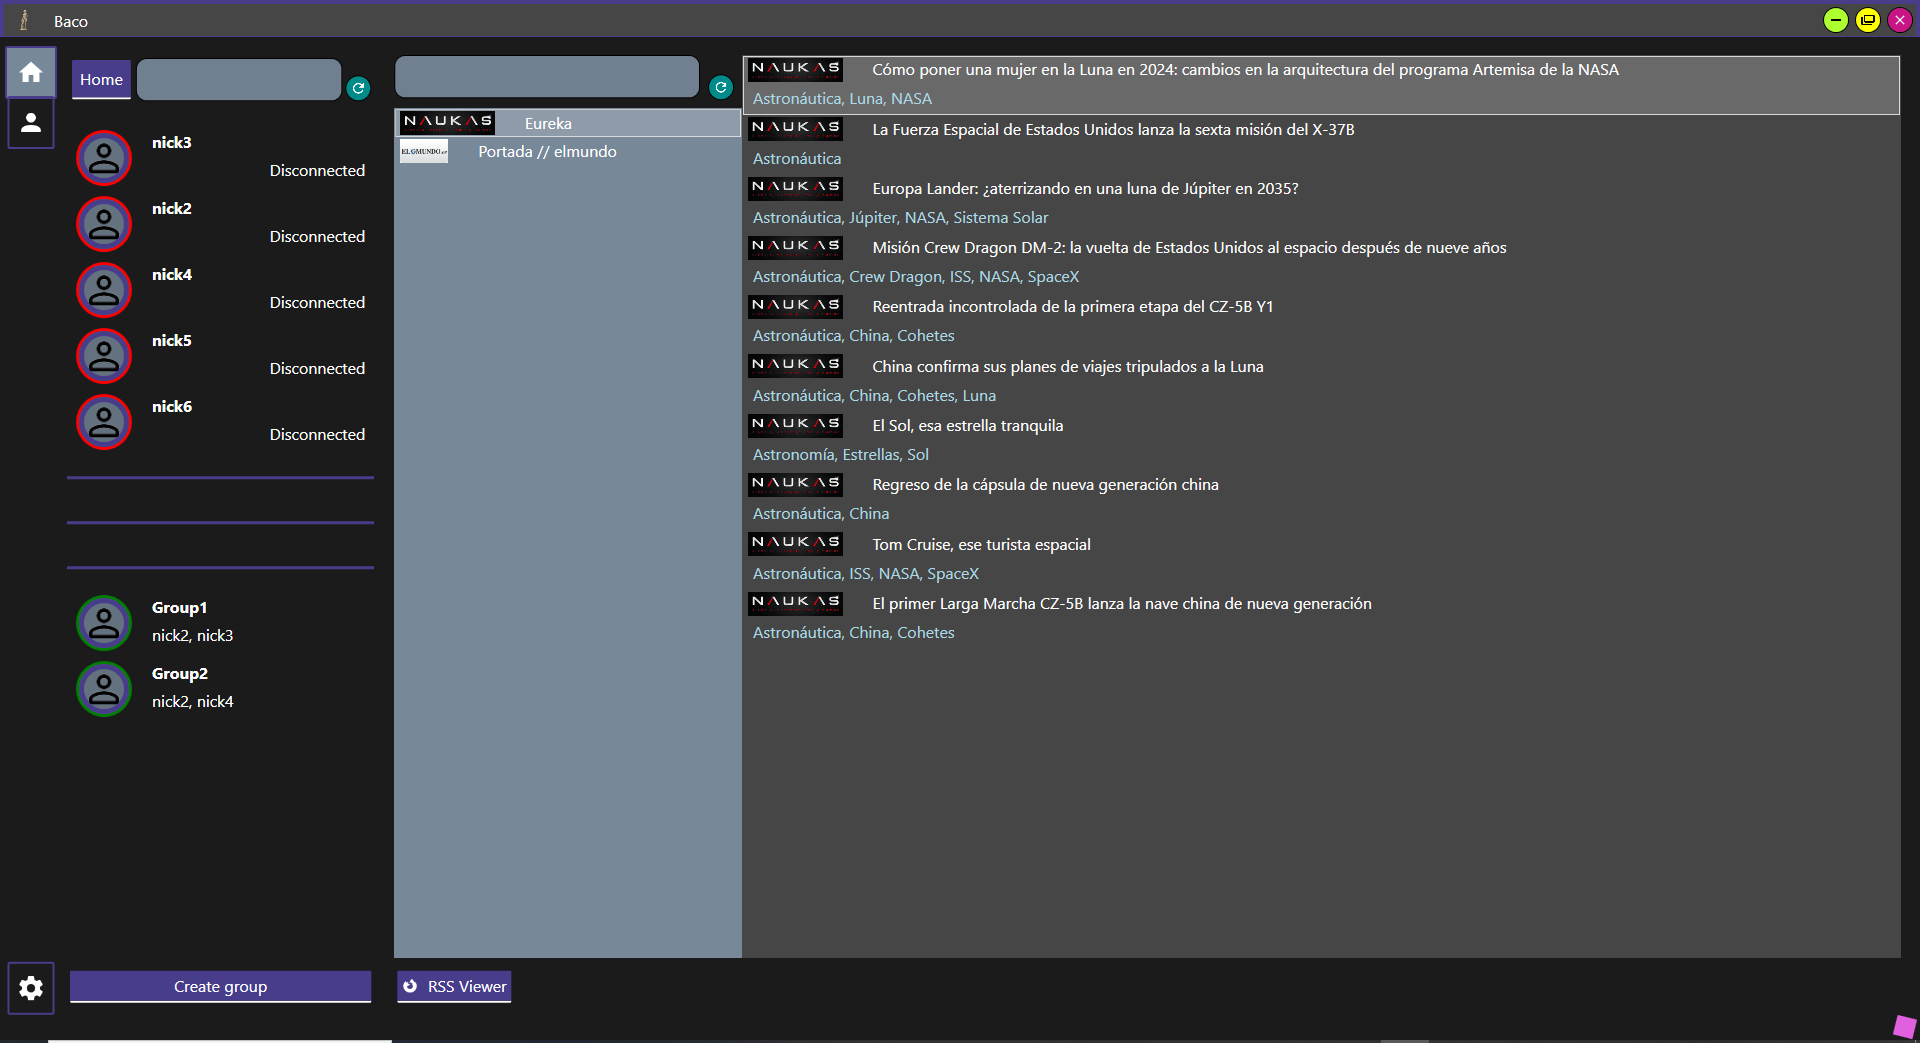
\includegraphics[width=\textwidth,height=0.3\textheight, keepaspectratio]{img/hub.PNG}
			\end{figure}
			
		\end{columns}
	\end{frame}

		\subsection{Comunicación cliente -- servidor}
		\begin{frame}{Comunicación cliente $\longrightarrow$ servidor}
			
			\note{Las comunicaciones que baco hace por medio de Internet son únicamente al servidor. Un cliente no puede acceder directamente al API REST, lo tiene que hacer mediante el servidor; esto lo veremos más adelante. La comunicación con el servidor se hace transmitiendo objetos de transporte serializables. Las funciones del servidor se verán más adelante.}

			\begin{tikzpicture}[level distance=0.4\textwidth]
			\node {Baco} [grow=right]
			child {node {Comunicación con el API REST}}
			child {node {Comunicación el servidor}
				child {node {Comunicación de estado}}
				child {node {Petición de datos}}
				child {node {Envío de mensajes}}
				child {node {Establecimiento de llamada}}
			};
			\end{tikzpicture}
		
		\end{frame}
	
		\subsection{Comunicación cliente -- base de datos}
		\begin{frame}{Comunicación cliente $\longrightarrow$ base de datos}
			
			\note{Aunque el cliente no pueda acceder directamente a la base de datos, sí que puede enviar peticiones a esta. En la siguiente diapositiva se extenderá este apartado. Las peticiones que se pueden hacer al API REST son las que se ven en pantalla:
			\begin{itemize}
				\item Validación de credenciales: cuando rellenamos los campos de inicio de sesión, la información introducida se valida aquí.
				\item Una vez validada la sesión se podrán realizar el resto de acciones, que creo que son bastante autoexplicativas.
			\end{itemize}}
			
			\begin{tikzpicture}[level distance=0.4\textwidth]
			\node {Baco} [grow=right]
			child {node {Comunicación con el API REST}	
				child {node {Obtener amigos}}
				child {node {Obtener suscripciones RSS}}
				child {node {Obtener grupos}}
				child {node {Obtener foto de perfil}}
				child {node {Validar credenciales}}
			}
			child {node {Comunicación el servidor}};
			\end{tikzpicture}
			
		\end{frame}

	\section{BacoServer -- Servidor}
	\begin{frame}{BacoServer -- Servidor}
		
		\note{El servidor de Baco tiene como propósito comunicar por Internet a los usuarios de la aplicación. Las acciones que puede realizar son las que se ven en pantalla:
		\begin{itemize}
			\item Registro de usuarios conectados: cuando un usuario entra al sistema, BacoServer lo registra como usuario conectado y notifica a todos sus amigos conectados.
			\item Control de llamadas: cuando las llamadas se establecen entre usuarios, BacoServer es el encargado de enviar a todos los usuarios de la llamada los datos (como el vídeo y la voz)
			\item Conexión al API REST: como anteriormente se ha comentado, los clientes no pueden acceder al API REST, en cierta forma no saben ni quién es. Si necesitan acceder a él lo harán por medio del servidor. De este modo la comunicación por red se simplifica: un cliente solamente tiene establecida la conexión con un servidor.
			\item Control sobre el propio servidor: gracias a que BacoServer tiene un sistema de comandos, nos permite realizar ciertas funciones como comprobar cuál es el estado de los usuarios conectados al servidor o reiniciarlo.
		\end{itemize}}
		
		\begin{columns}
			\column{0.5\textwidth}
			\begin{itemize}
				\item Registro de usuarios conectados
				\item Control de llamadas
			\end{itemize}
			\column{0.5\textwidth}
			\begin{itemize}
				\item Conexión al API REST
				\item Control sobre el propio servidor
			\end{itemize}
		\end{columns}
	\end{frame}

		\subsection{Comunicación servidor -- cliente}
		\begin{frame}{Comunicación servidor $\longrightarrow$ cliente}
			
			\note{La comunicación entre BacoServer y el cliente se da, principalmente, debido a peticiones del usuario, es decir, rara vez el servidor envía datos al cliente por él mismo, suele ser porque otro usuario quiere comunicarse con el cliente, ya sea por medio de un mensaje, una llamada o una simple petición de amistad. El único caso que el servidor envía algo por sí mismo al cliente es cuando hay algún error en su conexión con BacoServer; se envía al cliente un objeto y este tiene que responder (algo así como un \selectlanguage{english}\textit{I'm alive}\selectlanguage{spanish}). Si no hay respuesta se considera que ha habido un problema en el cliente y no tendría que estar conectado.}
			
			
			\begin{tikzpicture}[level distance=0.39\textwidth]
			\node {BacoServer} [grow=right]
			child {node {Comunicación con el API REST}}
			child {node {Comunicación el cliente}
				child {node {Envío de estado de amigos}}
				child {node {Devolución de datos (API REST)}}
				child {node {Envío de mensajes}}
				child {node {Envío de información}}
			};
			\end{tikzpicture}
		\end{frame}
	
		\subsection{Comunicación servidor -- base de datos} \label{sbs:comsrvbd}
		\begin{frame}{Comunicación servidor $\longrightarrow$ base de datos}
			
			\note{Podemos ver que, la comunicación del servidor con el API REST es exactamente la misma que la del cliente con este. Esto es debido a lo comentado anteriormente: el cliente accede al API REST mediante el servidor, por lo tanto el servidor hará las peticiones del cliente. No obstante se han de comentar dos casos en los que se realizan peticiones al API REST por iniciativa del servidor. Entendemos iniciativa como las peticiones que se realzian sin que un cliente haya desencadenado esa petición, por ejemplo, un usuario se conecta y el servidor envía una petición al API REST para obtener sus amigos, eso no sería iniciativa del servidor. Cuando el servidor se pone en marcha nos pide la localización del API REST. Cuando se introduce, el servidor por sí mismo hace una petición al API REST y espera su respuesta. Si no hay respuesta se comunica que no se ha podido establecer la comunicación. Una vez se haya establecido, el servidor pedirá al API REST los grupos existentes. Esto es porque los grupos en cierta forma, se manejan como usuarios en sí. No obstante, como los grupos no pueden conectarse, tenemos que obtener desde un principio cuáles son los grupos con los que puede haber comunicaciones. Debido a que la magnitud de este programa no es muy grande, los grupos se cargan en memoria.}
			
			\begin{tikzpicture}[level distance=0.39\textwidth]
			\node {BacoServer} [grow=right]
			child {node {Comunicación con el API REST}	
				child {node {Obtener amigos}}
				child {node {Obtener suscripciones RSS}}
				child {node {Obtener grupos}}
				child {node {Obtener foto de perfil}}
				child {node {Validar credenciales}}
			}
			child {node {Comunicación el servidor}};
			\end{tikzpicture}
		\end{frame}

	\section{API REST}
	\begin{frame}{API REST}
		
		\only<1>{ \note{Desde el API REST solo podremos hacer las acciones de \selectlanguage{english}\textit{GET}\selectlanguage{spanish}, \selectlanguage{english}\textit{PUT}\selectlanguage{spanish}, \selectlanguage{english}\textit{POST}\selectlanguage{spanish} y \selectlanguage{english}\textit{DELETE}\selectlanguage{spanish}.}
			\begin{tikzpicture}[grow cyclic, text width=0.8\textwidth, align=flush center,
			level 1/.style={level distance=2cm,sibling angle=90},
			level 2/.style={level distance=2cm,sibling angle=45}]
			\node {API REST}
			child {node {GET}}
			child {node {PUT}}
			child {node {POST}}
			child {node {DELETE}};
			\end{tikzpicture}}
		
		\only<2>{ \note{El más extenso es el \selectlanguage{english}\textit{GET}\selectlanguage{spanish}; en él podremos obtener todo cuanto aparece en pantalla. No obstante, las fotos de perfil no se encuentran en la base de datos, sino en disco, pero se puede acceder a ellas de forma normal.}
			\begin{tikzpicture}[grow cyclic, text width=2.7cm, align=flush center,
			level 1/.style={level distance=6cm,sibling angle=90},
			level 2/.style={level distance=3cm,sibling angle=35}]
		\node {API REST}
		child {node {GET}
			child {node {Usuarios}}
			child {node {Disponibilidad de correo electrónico}}
			child {node {Grupos}}
			child {node {Suscripciones}}
			child[style={level distance=4cm}] {node {Validaciones de inicio de sesión}}
			child {node {Búsqueda de amigos}}
			child {node {ID}} 
			child {node {Amigos}}
			child {node {Foto de perfil}}
		};
		\end{tikzpicture}}
	
		\only<3>{ \note{Las modificaciones a la base de datos son simples: se puede cambiar la foto de perfil, modificar amistades, responder peticiones de amistad y modificar usuarios.}
			\begin{tikzpicture}[grow cyclic, text width=2.7cm, align=flush center,
			level 1/.style={level distance=7cm,sibling angle=90},
			level 2/.style={level distance=3cm,sibling angle=45}]
			\node {API REST}
			child {node {PUT}
				child {node {Usuarios}}
				child {node {Peticiones de amistad}}
				child {node {Amigos}}
				child {node {Foto de perfil}} 
			};
		\end{tikzpicture}}
	
		\only<4>{ \note{En la base de datos se puede insertar la foto de perfil, un nuevo amigo y un usuario nuevo.}
			\begin{tikzpicture}[grow cyclic, text width=2.7cm, align=flush center,
			level 1/.style={level distance=7cm,sibling angle=90},
			level 2/.style={level distance=3cm,sibling angle=45}]
			\node {API REST}
			child {node {POST}
				child {node {Usuarios}}
				child[style={level distance=4cm}] {node {Amigos}}
				child {node {Foto de perfil}}
			};
		\end{tikzpicture}}
	
		\only<5>{ \note{Por el momento, Baco solamente tiene una acción de borrado: los usuarios.}
			\begin{tikzpicture}[grow cyclic, text width=2.7cm, align=flush center,
			level 1/.style={level distance=7cm,sibling angle=90},
			level 2/.style={level distance=3cm,sibling angle=45}]
			\node {API REST}
			child {node {DELETE}
				child[style={level distance=4cm}] {node {Usuario}}
		};
		\end{tikzpicture}}
	\end{frame}
	
\end{document}